\section{Geometrically Frustrated Systems}
\subsection{What is a Geometrically Frustrated System?}
Geometrically frustrated systems are systems in which multiple configurations give the same total energy.  A system exhibits this type of frustration when it is not possible to minimize the interaction energy between each of the elements of the system simultaneously. A degeneracy in the ground state is a characteristic of these frustrated systems. This degeneracy leads to an interesting effect, as the temperature of the system approaches zero the entropy reaches some finite value.
\par
\begin{figure}[ht!]
    \begin{center}
        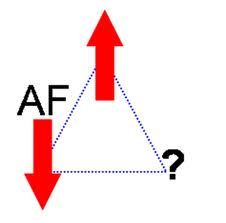
\includegraphics[scale=0.4]{trifrust.png}
        \caption[Triangular spin arrangement]{Frustration arising from anti-ferromagnetic interactions in a triangular spin arrangement}
        \label{fig:gf1}
    \end{center}
\end{figure}
The above figure is an example of one of the most basic examples of this frustration, consider 3 spins which interact via anti-ferromagnetic interaction placed at the corners of an equilateral triangle. In this triangular lattice geometry, to align the third spin such that it minimises its total interaction energy gives the exact same energy whether the third spin is +1 or -1.
\par
Why this occurs is because there is no way to orient the spin such that it minimizes it's interaction with the other two spins simultaneously resulting in a two-fold degenerate ground state. The existence of a degenerate ground state is a defining characteristic of a frustrated system. An important note to make here is that this kind of frustration is a result of the topology of a well-ordered system, rather than the result of a disorder in the system.  Hence why this is referred to as geometric frustration.
\par
\subsection{Geometrical Frustration in Water Ice}
An example of frustration in a system can be seen by looking at ordinary water ice at low temperature. When water ice was investigated experimentally in 1933 by W.F. Giauque \& M.F. Ashley, the entropy of ice at low temperatures did not agree with the predicted theoretical value. In fact, when the results were extrapolated toward absolute zero kelvin, it was found that the entropy of the system was non-zero.{\cite{b5}}
\par
This result appeared to be in direct contradiction to the famous third law of thermodynamics which states that entropy as a measure of the disorder of a system should approach zero as temperature approaches 0.  In 1935, Linus Pauling attributed this discrepancy to a frustration resulting from the geometric structure of the bonds between the oxygen and hydrogen atoms and thus the existence of a degenerate ground state.{\cite{b6}}
\par
The frustrated structure of the water ice occurs in the I$_{h}$ phase of water ice.{\cite{b7}}  H$^{2}$O molecules are arrayed in such a way that the bond angle from the liquid phase is almost preserved. Each oxygen ion is bonded covalently to four hydrogen ions or protons.
\par
However, the protons are not all positioned equidistant between the oxygen ions. Instead relative to each oxygen atom, the hydrogen atoms' positions are that two of the neighbouring hydrogen are relatively close and two relatively far away.  This arrangement gives the lowest energy configuration in each tetrahedral unit.
\par
\begin{figure}[ht!]
    \begin{center}
        \subfloat[Locations of protons][Locations of protons]{
        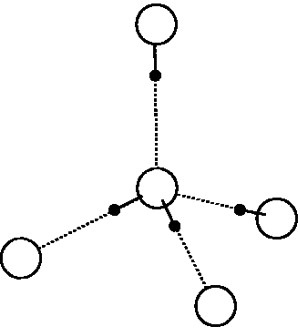
\includegraphics[width=0.3\textwidth]{2in2outex.png}
        \label{fig:sf2.1}}
\qquad
        \subfloat[Tetrahedral water ice lattice][Tetrahedral water ice lattice]{
        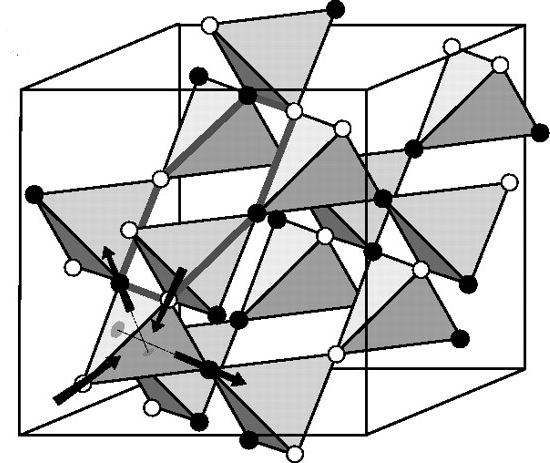
\includegraphics[width=0.3\textwidth]{pyrolat.png}
        \label{fig:sf2.2}}
        \caption{Structure of water ice.}
        \label{fig:gf2}
    \end{center}
\end{figure}
Figure 3(a) shows one such arrangement with the large white circles and small black circles representing oxygen and hydrogen respectfully.  Figure 3(b) is an example of how a segment of the lattice is constructed from the tetrahedral units.
\par
\begin{figure}[ht!]
    \begin{center}
        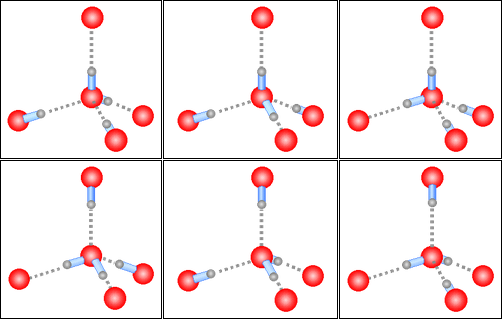
\includegraphics[scale=0.65]{hydroarrang.png}
        \caption[Tetrahedral unit configurations]{There are 6 different arrangements each tetrahedral unit can take on}
        \label{fig:gf3}
    \end{center}
\end{figure}
\par
This tendency toward a two-in, two-out configuration is known as the Bernal-Fowler ice rule.  Pauling showed that for a macroscopic number of atoms the ice rules lead to a 6-fold degeneracy in the ground state, even at zero temperature.  Thus the system is left with a residual entropy. Pauling calculated this residual entropy and it was in very good agreement with the extrapolated experimental value.
\par
Unfortunately, studying the properties of water ice specifically to see `monopole/anti-monopole' pairs is inherently difficult because of the need for immaculately pure crystals of water ice.  To put this into perspective, the water ice crystals needed would require purities rivalling that of modern silicon crystals used for semiconductors but with the added challenge of keeping the crystals at a structure preserving temperature and ensuring the temperature is uniform to a sufficient degree throughout the crystal.
\clearpage
\subsection{Spin Ice Structures}
There is however another material that has the same tetrahedral structure as water ice.  Philip Anderson realised this when he noticed there was a straightforward mapping between Pauling's water ice model and an anti-ferromagnetic two state Ising model on a pyrochloric lattice.{\cite{b10}}
\par
The problem with such a two state model is not that it would require all of the spins to point either parallel or anti-parallel to a single global z-axis but given there is no reason for the system to prefer this particular orientation over another in a magnetic material exhibiting global cubic symmetry makes this a physically unrealistic model.
\par
In a paper published in 1997, it was discovered that there was a mapping between the water ice model and a ferromagnetic, rather than anti-ferromagnetic, two state Ising model, also on a pyrochloric lattice. However, there is a difference from the previous mapping in that the spins must be constrained to point either toward or away from the centre of the tetrahedron.
\par
\begin{figure}[ht!]
    \begin{center}
        \subfloat[Collinear Spins][Collinear Spins]{
        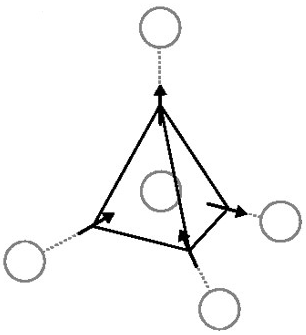
\includegraphics[width=0.3\textwidth]{spindir2i2o.png}
        \label{fig:sf4.1}}
\qquad
        \subfloat[Non-Collinear Spins][Non-Collinear Spins]{
        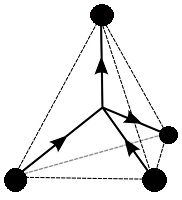
\includegraphics[width=0.3\textwidth]{spindir2i2onc.png}
        \label{fig:sf4.2}}
        \caption[Tetrahedral unit spin configurations]{Tetrahedral unit spin configurations}
        \label{fig:gf4}
    \end{center}
\end{figure}
In the above Figure 5. the tetrahedrals outlined in both figures correspond directly with each other but Figure (b) has striped the neighbouring oxygen atoms to make it easier to visualize the orientation of the hydrogen spins. It is clear from this picture that the spin axis are collinear in (a) yet in (b) they are non-collinear.  Figure (b) shows a strong magnetic anisotropy or preference for the spins to point along the axis which connects a spin to the center of it's tetrahedron. In crystallography this is known as the $<$111$>$ axis.
\par
In this model, the degenerate ground states of a single tetrahedron  obeys the ice rule, with two spins pointing in and two pointing out. M.J. Harris and his team referred to the model as the `spin ice model' and experimentally observed it to be approximated by the magnetic pyrochlore oxide Ho$_{2}$Ti$_{2}$O$_{7}$.{\cite{b11}.
\par
This frustration arising from ferromagnetic interactions is quite unexpected, yet the experimental value for the residual entropy of the spin ice Dy$_{2}$Ti$_{2}$O$_{7}$ investigated by A.P. Ramirez et al. in 1999 was been found to agree reasonably well with Pauling's value for the residual entropy of water ice.{\cite{b12} This is direct experimental evidence for the existence of a macroscopically degenerate ground state and an ice-rule obeying spin ice ground state.
\clearpage
